%----------------------------------------------------------------------------------------
%	PACKAGES AND OTHER DOCUMENT CONFIGURATIONS
%----------------------------------------------------------------------------------------

\documentclass{article}

\usepackage{fancyhdr} % Required for custom headers
\usepackage{lastpage} % Required to determine the last page for the footer
\usepackage{extramarks} % Required for headers and footers
\usepackage[usenames,dvipsnames]{color} % Required for custom colors
\usepackage{graphicx} % Required to insert images
\usepackage{subcaption}
\usepackage{listings} % Required for insertion of code
\usepackage{courier} % Required for the courier font
\usepackage{lipsum} % Used for inserting dummy 'Lorem ipsum' text into the template
\usepackage{amsmath}
\usepackage{float}

% Margins
\topmargin=-0.45in
\evensidemargin=0in
\oddsidemargin=0in
\textwidth=6.5in
\textheight=9.0in
\headsep=0.25in

\linespread{1.1} % Line spacing

% Set up the header and footer
\pagestyle{fancy}
\lhead{\hmwkAuthorName} % Top left header
\chead{\hmwkClass\ : \hmwkTitle} % Top center head
%\rhead{\firstxmark} % Top right header
\lfoot{\lastxmark} % Bottom left footer
\cfoot{} % Bottom center footer
\rfoot{Page\ \thepage\ of\ \protect\pageref{LastPage}} % Bottom right footer
\renewcommand\headrulewidth{0.4pt} % Size of the header rule
\renewcommand\footrulewidth{0.4pt} % Size of the footer rule

\setlength\parindent{0pt} % Removes all indentation from paragraphs


%----------------------------------------------------------------------------------------
%	DOCUMENT STRUCTURE COMMANDS
%	Skip this unless you know what you're doing
%----------------------------------------------------------------------------------------

% Header and footer for when a page split occurs within a problem environment
\newcommand{\enterProblemHeader}[1]{
	%\nobreak\extramarks{#1}{#1 continued on next page\ldots}\nobreak
	%\nobreak\extramarks{#1 (continued)}{#1 continued on next page\ldots}\nobreak
}

% Header and footer for when a page split occurs between problem environments
\newcommand{\exitProblemHeader}[1]{
	%\nobreak\extramarks{#1 (continued)}{#1 continued on next page\ldots}\nobreak
	%\nobreak\extramarks{#1}{}\nobreak
}

\setcounter{secnumdepth}{0} % Removes default section numbers
\newcounter{homeworkProblemCounter} % Creates a counter to keep track of the number of problems
\setcounter{homeworkProblemCounter}{0}

\newcommand{\homeworkProblemName}{}
\newenvironment{homeworkProblem}[1][Problem \arabic{homeworkProblemCounter}]{ % Makes a new environment called homeworkProblem which takes 1 argument (custom name) but the default is "Problem #"
	\stepcounter{homeworkProblemCounter} % Increase counter for number of problems
	\renewcommand{\homeworkProblemName}{#1} % Assign \homeworkProblemName the name of the problem
	\section{\homeworkProblemName} % Make a section in the document with the custom problem count
	\enterProblemHeader{\homeworkProblemName} % Header and footer within the environment
}{
	\exitProblemHeader{\homeworkProblemName} % Header and footer after the environment
}

\newcommand{\problemAnswer}[1]{ % Defines the problem answer command with the content as the only argument
	\noindent\framebox[\columnwidth][c]{\begin{minipage}{0.98\columnwidth}#1\end{minipage}} % Makes the box around the problem answer and puts the content inside
}

\newcommand{\homeworkSectionName}{}
\newenvironment{homeworkSection}[1]{ % New environment for sections within homework problems, takes 1 argument - the name of the section
	\renewcommand{\homeworkSectionName}{#1} % Assign \homeworkSectionName to the name of the section from the environment argument
	\subsection{\homeworkSectionName} % Make a subsection with the custom name of the subsection
	\enterProblemHeader{\homeworkProblemName\ [\homeworkSectionName]} % Header and footer within the environment
}{
	\enterProblemHeader{\homeworkProblemName} % Header and footer after the environment
}


%========================================================================================================
%----------------------------------------------------------------------------------------
%	NAME AND CLASS SECTION
%----------------------------------------------------------------------------------------

\newcommand{\hmwkTitle}{Assignment\ \#3} % Assignment title
\newcommand{\hmwkClass}{CSC321} % Course/class
\newcommand{\hmwkAuthorName}{Xiangyu Kong} % Your name
\newcommand{\hmwkUTorId}{kongxi16} % UTorID

%----------------------------------------------------------------------------------------
%	TITLE PAGE
%----------------------------------------------------------------------------------------

\title{
	\vspace{2in}
	\textmd{\textbf{\hmwkClass:\ \hmwkTitle}}\\
	%	\normalsize\vspace{0.1in}\small{Due\ on\ \hmwkDueDate}\\
	\vspace{0.1in}
	\vspace{3in}
}

\author{\textbf{\hmwkAuthorName} \\ \textbf{\hmwkUTorId}}

% Insert date here if you want it to appear below your name
\date{\today} 

%----------------------------------------------------------------------------------------

\begin{document}
	
	\maketitle
	\clearpage
	
	
	%---------------------------------------------------------------------------------
	%	PROBLEM 1
	%---------------------------------------------------------------------------------
	
	\begin{homeworkProblem}
		\begin{align*}
			\mathbf{W}^{(1)} &= \begin{bmatrix}
											-1 & 1 & 0 & 0 \\
											0 & -1 & 1 & 0 \\
											0 & 0 & -1 & 1
											\end{bmatrix}\\
			\mathbf{b}^{(1)} &= \begin{bmatrix}
											0 \\
											0 \\
											0
											\end{bmatrix}\\
			\mathbf{w}^{(2)} &= \begin{bmatrix}
											1 \\
											1 \\
											1
											\end{bmatrix}\\
			b^{(2)} &= -2.5
		\end{align*}
		
	\end{homeworkProblem}
	\clearpage
	
	
	
	%---------------------------------------------------------------------------------
	%	PROBLEM 2
	%---------------------------------------------------------------------------------
	
	\begin{homeworkProblem}
		\begin{enumerate}
			\item As shown in Figure 1
			\begin{figure}[H]
				\centering
				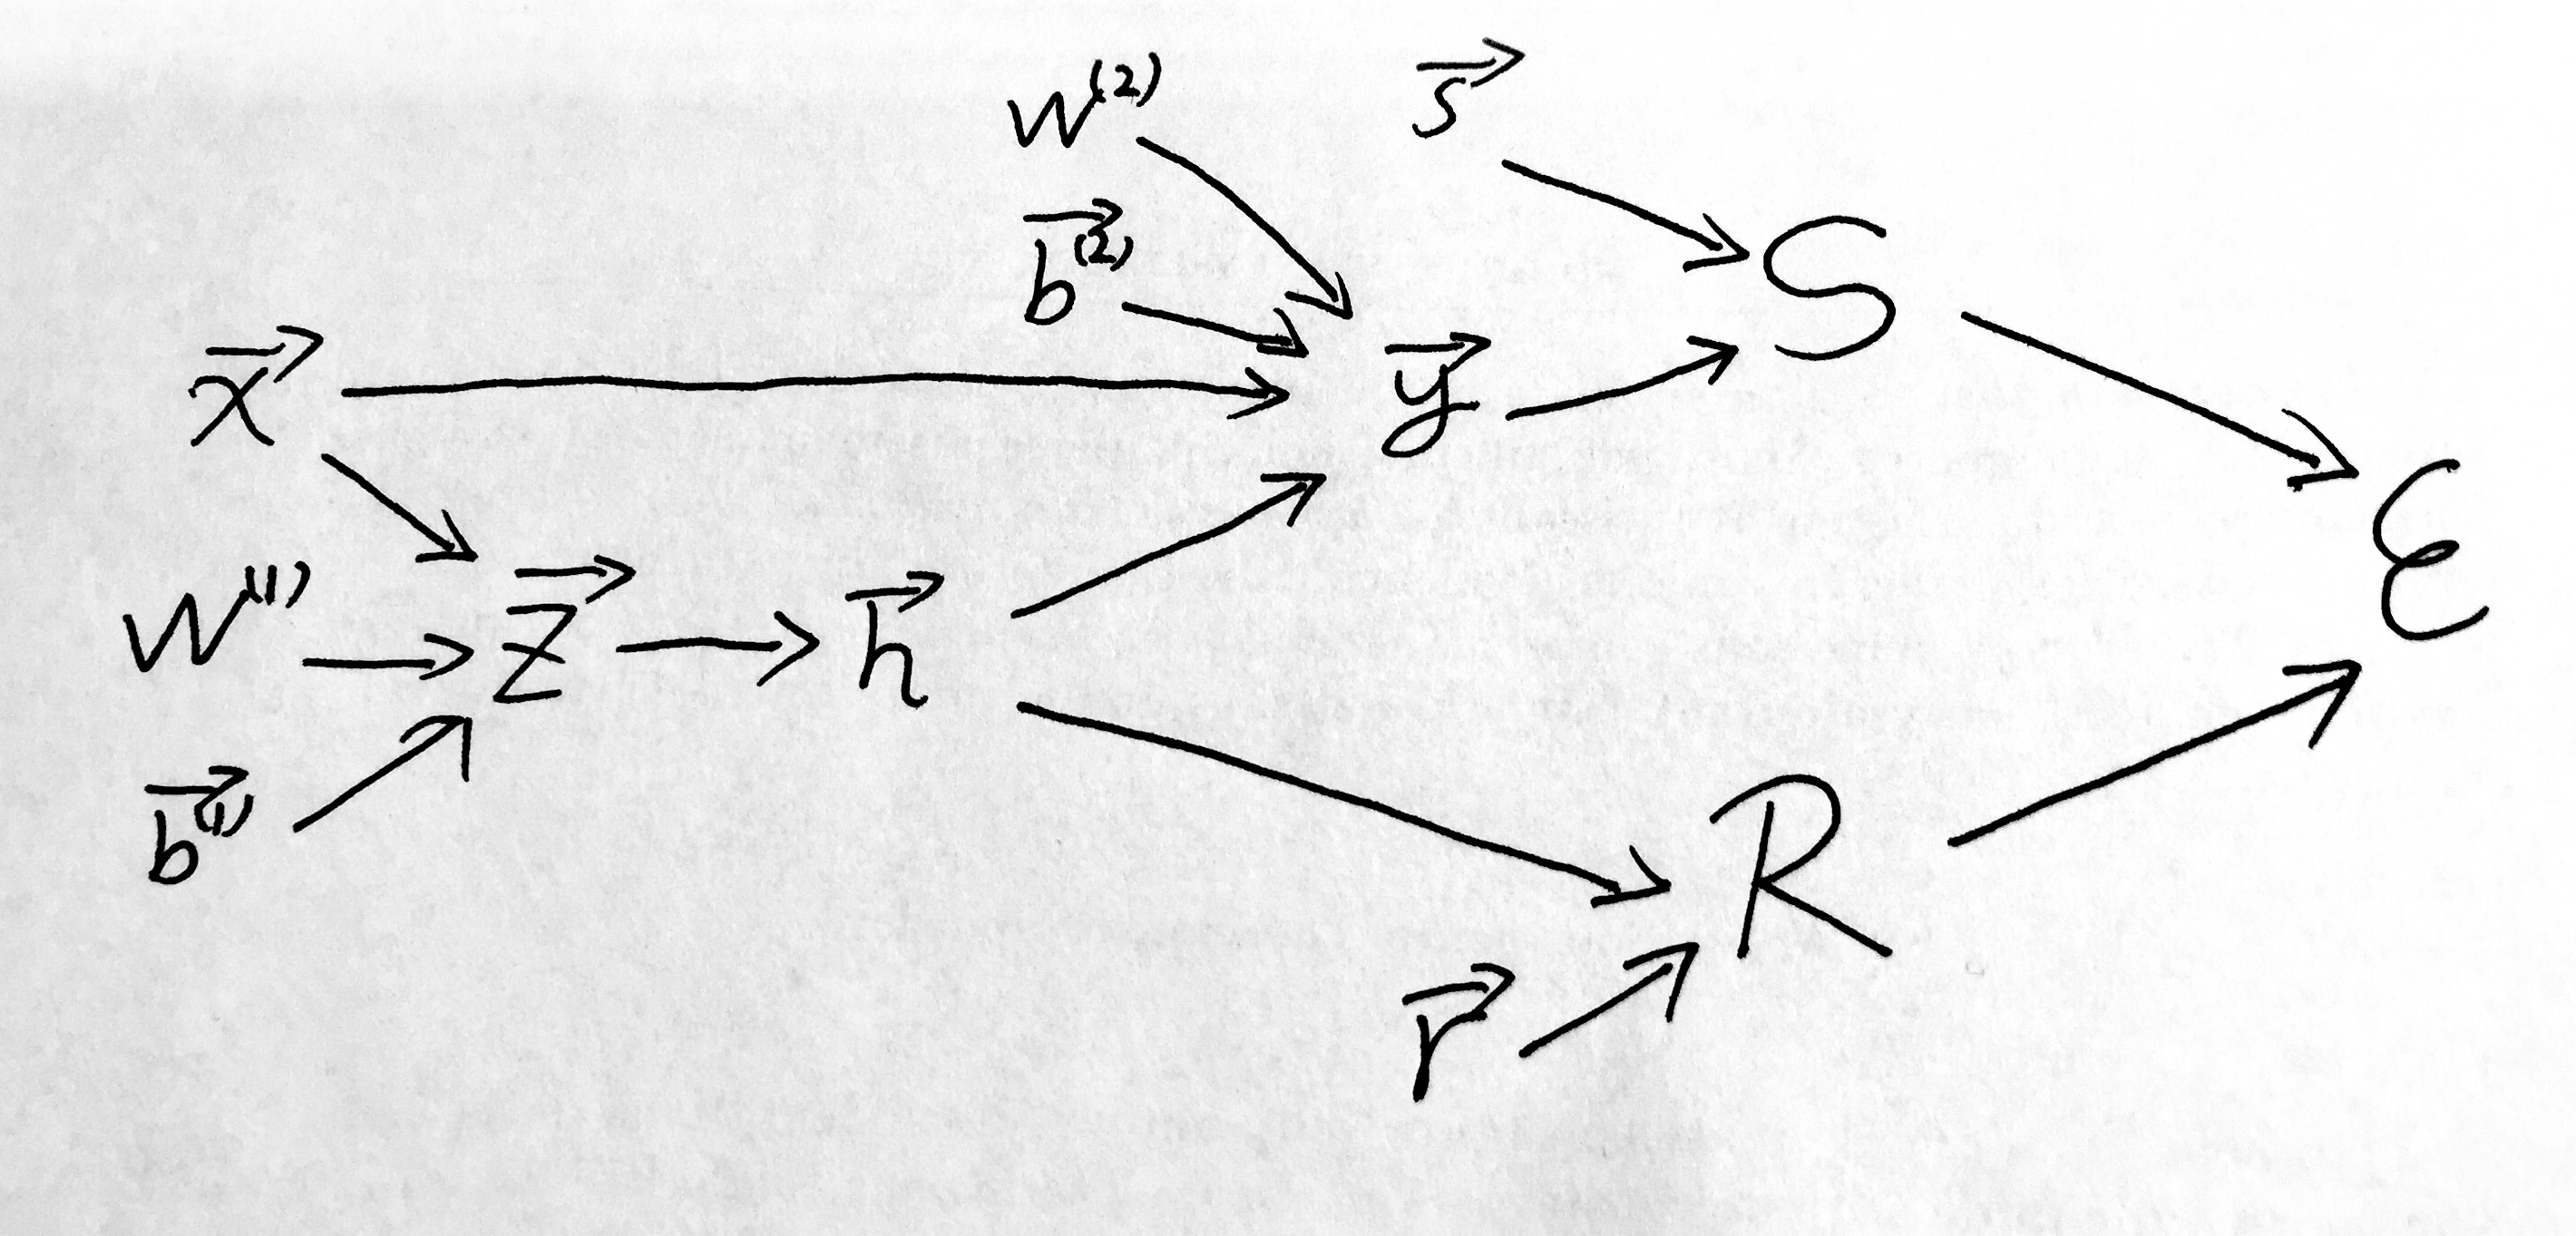
\includegraphics[width=.5\linewidth]{1.jpg}
				\caption{2.1 \label{}}
			\end{figure}
			
			\item 
			\begin{align*}
				\overline{\mathcal{E}} &= 1\\
				\overline{\mathcal{S}} &= \overline{\mathcal{E}} \dfrac{d\mathcal{E}}{d\mathcal{S}} = 1\\
				\overline{\mathcal{R}} &= \overline{\mathcal{E}} \dfrac{d\mathcal{E}}{d\mathcal{R}} = 1\\
				\overline{\mathbf{y}} &= \overline{\mathcal{S}} \dfrac{d\mathcal{S}}{d\mathbf{y}} = 
					1 ||\mathbf{y} - \mathbf{s}|| = ||\mathbf{y} - \mathbf{s}||\\
				\overline{\mathbf{h}} &= \overline{\mathbf{y}} \dfrac{d\mathbf{y}}{d\mathbf{h}} +
					 \overline{\mathcal{R}} \dfrac{d\mathcal{R}}{d\mathbf{h}} = 
					 ||\mathbf{y} - \mathbf{s}|| \mathbf{W}^{(2)'} + \mathbf{r}^{\top'}\\
				\overline{\mathbf{z}} &= \overline{\mathbf{h}} \dfrac{d\mathbf{h}}{d\mathbf{z}} =
					(||\mathbf{y} - \mathbf{s}|| \mathbf{W}^{(2)'} + 
					\mathbf{r}^{\top'}) \sigma'(\mathbf{z})\\
				\overline{\mathbf{x}} &= \overline{\mathbf{z}} \dfrac{d\mathbf{z}}{d\mathbf{x}} +
					\overline{\mathbf{y}} \dfrac{d\mathbf{y}}{d\mathbf{x}} = 
					(||\mathbf{y} - \mathbf{s}|| \mathbf{W}^{(2)'} + 
					\mathbf{r}^{\top'}) \sigma'(\mathbf{z}) \mathbf{W}^{(1)'} + ||\mathbf{y} - \mathbf{s}||
			\end{align*}
		\end{enumerate}
		
		
	\end{homeworkProblem}
	\clearpage
	
	
	%---------------------------------------------------------------------------------
	%	PROBLEM 3
	%---------------------------------------------------------------------------------
	
	\begin{homeworkProblem}
		\begin{enumerate}
			\item 
			$\dfrac{\partial \mathcal{L}}{\partial w_1}$: YES\\
			Using back-propagation:\\
			\begin{align*}
				\overline{\mathcal{L}} &= 1\\
				\overline{y} &= \overline{\mathcal{L}} \dfrac{d \mathcal{L}}{d y} = f'(y)\\
				\overline{w_1} &= \overline{y} \dfrac{d y}{d w_1} = f'(y) 0 = 0
			\end{align*}
			
			\item 
			$\dfrac{\partial \mathcal{L}}{\partial w_2}$: NO\\
			Using back-propagation:\\
			\begin{align*}
				\overline{\mathcal{L}} &= 1\\
				\overline{y} &= \overline{\mathcal{L}} \dfrac{d \mathcal{L}}{d y} = f'(y)\\
				\overline{h_1} &= \overline{y} \dfrac{d y}{d h_1} = f'(y) w_1\\
				\overline{w_2} &= \overline{h_1} \dfrac{d h_1}{d h_1} = f'(y) w_1 h_3
			\end{align*}
			If $f'(y) w_1 h_3 \neq 0$, 	$\dfrac{\partial \mathcal{L}}{\partial w_2}$ does not necessarily equal to 0.
			
			\item 
			$\dfrac{\partial \mathcal{L}}{\partial w_3}$: NO\\
			Using back-propagation:\\
			\begin{align*}
			\overline{\mathcal{L}} &= 1\\
			\overline{y} &= \overline{\mathcal{L}} \dfrac{d \mathcal{L}}{d y} = f'(y)\\
			\overline{h_1} &= \overline{y} \dfrac{d y}{d h_1} = f'(y) w_1\\
			\overline{h_3} &= \overline{h_1} \dfrac{d h_1}{d h_3} = f'(y) w_1 w_3\\
			\overline{w_3} &= \overline{h_3} \dfrac{d h_3}{d w_3} = f'(y) w_1 w_3 x_1
			\end{align*}
			If $f'(y) w_1 w_3 x_1 \neq 0$, 	$\dfrac{\partial \mathcal{L}}{\partial w_3}$ does not necessarily equal to 0.
		\end{enumerate}
		
	\end{homeworkProblem}
	\clearpage
	
	%----------------------------------------------------------------------------------------
	
\end{document}